% Illustration artwork with separately maintained, code-checked vector wiring.
\definecolor{FlowBlue}{HTML}{2166AC}
\definecolor{FlowRed}{HTML}{B2182B}
\begin{tikzpicture}[x=.01cm,y=-.01cm,>=Latex,
 flow/.style={->,draw=black!75,line width=.5pt},
 init/.style={->,draw=black!45,dashed,line width=.5pt,preaction={draw=white,line width=1.6pt,-}},
 ref/.style={->,draw=FlowBlue,dashed,line width=.55pt,preaction={draw=white,line width=1.6pt,-}},
 update/.style={->,draw=FlowRed,line width=.6pt,preaction={draw=white,line width=1.6pt,-}},
 small/.style={font=\fontsize{4.5}{5.3}\selectfont,fill=white,inner sep=.7pt}]
\node[anchor=north west,inner sep=0] at (0,0)
 {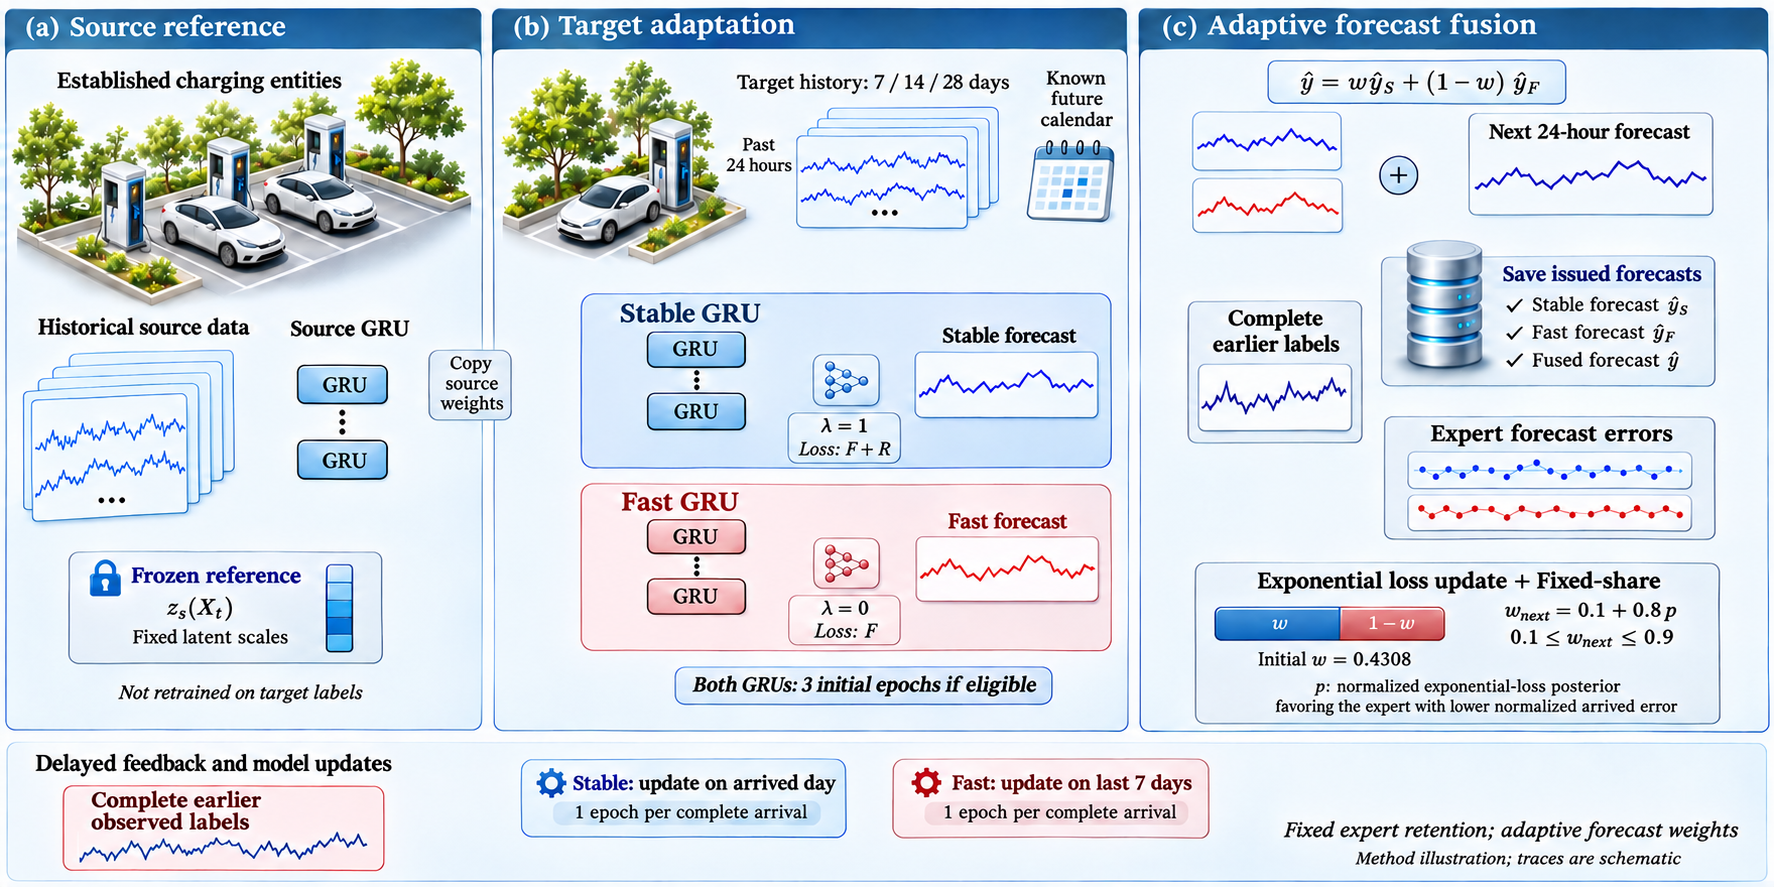
\includegraphics[width=17.74cm]{figures/illustrated-system-artwork-v1.png}};
% (a) Source training, copied parameters, and a separate frozen reference.
\draw[flow] (235,433)--(270,433)--(270,385)--(297,385);
\draw[flow,preaction={draw=white,line width=2pt,-}] (342,406)--(342,440);
\draw[flow] (387,460)--(410,460)--(410,385)--(428,385);
\draw[flow] (342,480)--(342,522)--(260,522)--(260,551);
\node[small] at (130,533) {same $X_t$};
\draw[flow] (130,541)--(130,551);
% (b) A black bus supplies the same permitted inputs to BOTH encoders.
\draw[flow] (871,229)--(871,252)--(529,252)--(529,349)--(647,349);
% Future calendar bypasses the encoder and enters BOTH calendar-aware heads.
\draw[flow] (1072,223)--(1072,271)--(897,271)--(897,342)--(847,342)--(847,353);
\draw[flow,preaction={draw=white,line width=1.6pt,-}] (897,342)--(897,527)--(847,527)--(847,538);
\fill[black!75] (897,342) circle (2.1);
\node[small] at (924,273) {$C_t$};
\draw[flow] (529,349)--(529,538)--(647,538);

\fill[black!75] (529,349) circle (2.1);
% Grey dashed parameter transfer stays distinct from the black input bus.
\draw[init] (512,385)--(555,385)--(555,321)--(581,321);
\draw[init] (555,385)--(555,502)--(581,502);
\fill[black!45] (555,385) circle (2);
% Schematic two-layer encoders and calendar-aware prediction heads.
\draw[flow,preaction={draw=white,line width=2pt,-}] (697,368)--(697,394);
\draw[flow] (745,412)--(783,412)--(783,380)--(813,380);
\draw[flow,preaction={draw=white,line width=1.6pt,-}] (880,380)--(913,380);
\draw[flow] (697,430)--(697,437)--(786,437);
\draw[flow,preaction={draw=white,line width=2pt,-}] (697,557)--(697,579);
\draw[flow] (745,596)--(785,596)--(785,565)--(813,565);
\draw[flow] (880,565)--(913,565);
% Frozen-source information enters the RETENTION LOSS, not a GRU input port.
\draw[ref] (359,600)--(566,600)--(566,449)--(786,449);
\node[small,text=FlowBlue] at (471,602) {$z_s(X_t),s$};
% (c) The two expert forecasts enter weighted fusion and are persisted.
\draw[flow] (1099,385)--(1148,385)--(1148,142)--(1193,142);
\draw[flow] (1099,570)--(1166,570)--(1166,204)--(1193,204);
\draw[flow] (1343,142)--(1367,142)--(1384,164);
\draw[flow] (1343,204)--(1367,204)--(1384,187);
\draw[flow] (1399,103)--(1399,156);
\draw[flow] (1419,176)--(1468,176);
\draw[flow] (1585,215)--(1585,255);
% Independent observations and saved expert forecasts meet ONLY at scoring.
\draw[flow] (1354,388)--(1374,388)--(1374,478)--(1384,478);
\draw[flow] (1551,385)--(1551,416);
\draw[flow] (1551,540)--(1551,563);
\draw[update] (1720,641)--(1742,641)--(1742,81)--(1567,81);
% Delayed labels supply both training policies, each returning to its own model.
\draw[update] (383,822)--(455,822)--(455,793)--(520,793);
\draw[update] (455,822)--(455,858)--(1058,858)--(1058,838);
\fill[FlowRed] (455,822) circle (2);
\draw[update,draw=FlowBlue] (680,759)--(680,735)--(579,735)--(579,412)--(647,412);
\draw[update] (1040,759)--(1040,733)--(661,733)--(661,614);
\end{tikzpicture}
